\documentclass[10pt, pscyr, nonums]{hedlabwork}
\usepackage[russian]{babel}
\usepackage{hedmaths}
\usepackage{graphicx}
\graphicspath{{images/}, {plots/}}

\labnum{606}
\labname{Изучение работы счетчика Гейгера-Мюллера}
\student{} \date{}

\newgeometry{top=1.5cm, bottom=1.5cm, left=1cm, right=1cm}
\begin{document}
  \makeheader

  \emph{Цель работы:} ознакомление с аппаратурой и методикой, применяемой при
    регистрации заряженных частиц, изучение взаимодействия \( \alpha \),
    \( \beta \) и \( \gamma \) излучения с веществом.

  \begin{figure}[h!]
    \center
    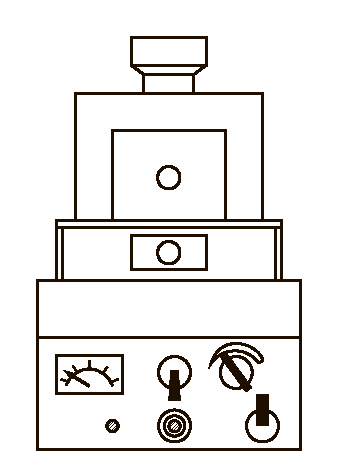
\includegraphics[width=.3\textwidth]{appearance} \\
      \parbox{.5\textwidth}{\caption{Внешний вид установки}}
  \end{figure}

  \begin{table}[h!]
    \center
    \caption{Определение фона космического излучения}
    \begin{tabular}{|*{4}{C{.2}|}} \hline
      Время счета, мин &
        Количество зарегистрированных импульсов \( N \) &
        Фон \( n_\varphi \), имп/мин &
        Среднее значение фона \( \midnum{n}_\varphi \), имп/мин \\ \hline
        &&& \multirow{3}{*}{} \\ \cline{1-2}
        &&& \\ \cline{1-2}
        &&& \\ \hline
    \end{tabular}
  \end{table}

  \begin{table}[h!]
    \center
    \caption{Определение счетной характеристики газоразрядного счетчика}
    \begin{tabular}{|C{.15}|*{4}{C{.1}|}} \hline
      Напряжение на счетчике \( V \),~В &
        \multicolumn{3}{C{.3}|}{Количество импульсов, зарегистрированных за 1~мин 
        \( n_0' \)} & \( \midnum{n_0'} \) \\ \hline
      260 &&&& \\ \hline
      280 &&&& \\ \hline
      300 &&&& \\ \hline
      320 &&&& \\ \hline
      340 &&&& \\ \hline
      360 &&&& \\ \hline
      380 &&&& \\ \hline
      400 &&&& \\ \hline
    \end{tabular}
  \end{table}

  \begin{table}[h!]
    \center
    \caption{Определение коэффициента поглощения алюминия}
    \begin{tabular}{|*{6}{C{.13}|}} \hline
      Толщина поглотителя,~мм &
        Количество импульсов, \( N_1 \) &
        Интервал счета, мин &
        Скорость счета \( n_1 \),~имп/мин &
        \( \dfrac{n_0}{n_1} \) &
        \( \ln\dfrac{n_0}{n_1} \) \\ \hline
      &&&&& \\ \hline
      &&&&& \\ \hline
      &&&&& \\ \hline
      &&&&& \\ \hline
      &&&&& \\ \hline
      &&&&& \\ \hline
    \end{tabular}
  \end{table}
  \pagebreak

  \subsection{Подсчет погрешности и окончательные результаты}
  \center
  \rule{.95\textwidth}{.5pt} \\ \rule{.95\textwidth}{.5pt}
  \rule{.95\textwidth}{.5pt} \\ \rule{.95\textwidth}{.5pt}
  \rule{.95\textwidth}{.5pt} \\ \rule{.95\textwidth}{.5pt}
  \rule{.95\textwidth}{.5pt} \\ \rule{.95\textwidth}{.5pt}
  \rule{.95\textwidth}{.5pt} \\ \rule{.95\textwidth}{.5pt} \\
  \vspace*{2em}

  \emph{Вывод:} \rule{.885\textwidth}{.5pt}
  \rule{.95\textwidth}{.5pt} \\ \rule{.95\textwidth}{.5pt}
  \rule{.95\textwidth}{.5pt}
\end{document}
